% !TeX root = ../D4.2a_User_Manual.tex
% !TeX spellcheck = en_GB

\section{Using the Separate Modelling and Simulation Tools}\label{sec:simulators}
This section provides a tutorial introduction to the FMI-specific functionality of each of the modelling and simulation tools.
%
This functionality is centered on the role of FMUs for each tool.
%
For more general descriptions of each tool, please refer to Appendix~\ref{appendix:tools}.
%
%
%
\subsection{Overture}
\label{sec:simulators:overture}
% !TeX root = D4.1a_User_Manual.tex
Overture implements export of both tool-wrapper as well as standalone FMUs.
%
It also has the ability to import a \texttt{model\-Description.\allowbreak{}xml} file in order to facilitate creating an FMI-compliant model from scratch.
%
A typical workflow in creating a new FMI-compliant VDM-RT model starts with the import of a \texttt{model\-Description.\allowbreak{}xml} file created using Modelio.
%
This results in a minimal project that can be exported as an FMU.
%
The desired model is then developed in this context.
%
This section discusses the complete workflow.
%
%
%
\subsubsection{Installing the FMI import/export plugin for Overture}
In order to use the FMI integration in Overture it is necessary to install a plugin.
Below is a guide to install the plugin:
\begin{enumerate}
	\item Open Overture.
	\item Select \textit{Help} -> \textit{Install New Software}.
	\item Click \textit{Add..}.
	\item In the \textit{Name:} field write \textit{Overture FMU}.
	\item In the \textit{Location:} field there are two options:
		\begin{description}
			\item[INTO-CPS Application:] Download the \textit{Overture FMU Import / Exporter - Overture FMI Support} using the Download Manager mentioned in Section \ref{sub:other-features}. Locate the file using the \textit{Archive...} button next to the \textit{Location:} field.
			\item[Update site:] Enter the following URL in the \textit{Location:} field: \\ \textit{http://overture.au.dk/into-cps/vdm-tool-wrapper/master/latest}.
		\end{description}
	\item Check the box next to \textit{Overture FMI Integration} as shown in Figure \ref{fig:importFMIoverture}.
	\item Click \textit{Next} or \textit{Finish} to accept and install.
\end{enumerate}
\begin{figure}[ht]
	\centering
	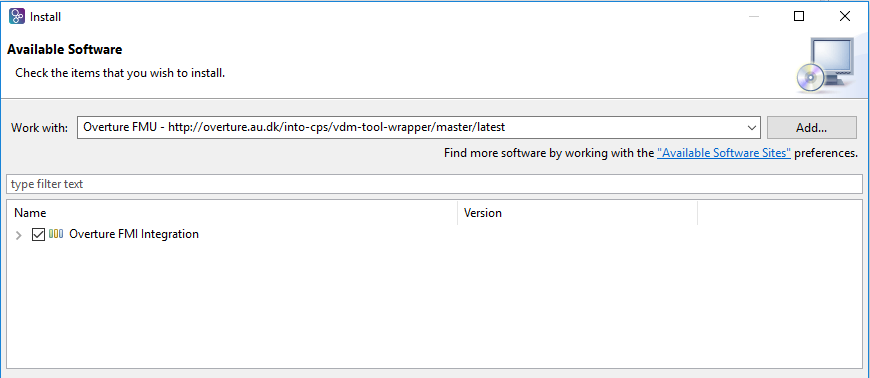
\includegraphics[width=5in]{figures/installOvertureFmiIntegration.png}
	\caption{Installing Overture FMI Integration.}
	\label{fig:importFMIoverture}
\end{figure}
%
%
%
\subsubsection{Import of \texttt{model\-Description.\allowbreak{}xml} File}
A \texttt{model\-Description.\allowbreak{}xml} file is easily imported into an existing, typically blank, VDM-RT project from the project explorer context menu as shown in Figure \ref{fig:moddescimportoverture}.
%
%
%
\begin{figure}[ht]
\centering
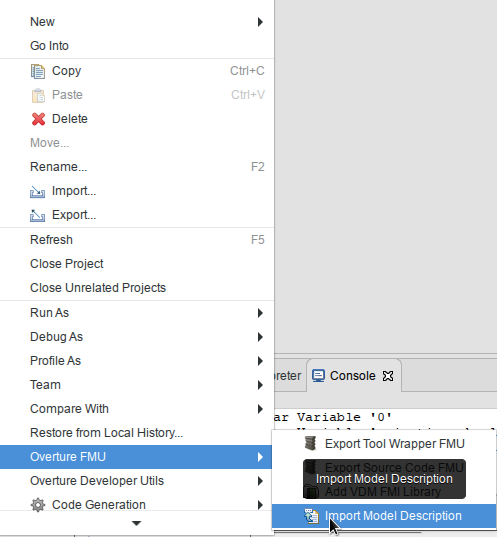
\includegraphics[width=3.7in]{figures/modelDescImportOverture.png}
\caption{Importing a \texttt{model\-Description.\allowbreak{}xml} file.}
\label{fig:moddescimportoverture}
\end{figure}
%
%
%
This results in the project being populated with the classes necessary for FMU export:
%
%
%
\begin{itemize}
\item  A VDM-RT \texttt{system} class named ``System'' containing the system definition.  The corresponding ``System'' class for the water tank controller FMU is shown in Listing \ref{lst:wtSystem}.
%
\item  A standard VDM-RT class named ``World''.  This class is conventional and only provides an entry point into the model.  The corresponding ``World'' class for the water tank controller FMU is shown in Listing \ref{lst:wtWorld}.
%
\item  A standard VDM-RT class named ``HardwareInterface''.  This class contains the definition of the input and output ports of the FMU.  Its structure is enforced, and a self-documenting annotation scheme\footnote{The annotation scheme is documented on the INTO-CPS website \url{into-cps-association.github.io} under ``\textit{Constituent Model Development} $\rightarrow$ \textit{Overture} $\rightarrow$ \textit{FMU Import/Export}.} is used such that the ``HardwareInterface'' class may be hand-written.  The corresponding ``HardwareInterface'' class for the water tank controller FMU is shown in Listing \ref{lst:wtHWInterface}.
%
\item  The library file \texttt{Fmi.vdmrt} which defines the hardware interface port types used in ``HardwareInterface''.
\end{itemize}
%
%
%
\begin{figure}[ht]
\begin{vdmrt}
system System

instance variables

-- Hardware interface variable required by FMU Import/Export
public static hwi: HardwareInterface := new HardwareInterface();
    

instance variables

  public levelSensor : LevelSensor;
  public valveActuator : ValveActuator;
  public static controller : [Controller] := nil;

	cpu1 : CPU := new CPU(<FP>, 20);
operations

public System : () ==> System
System () == 
(
	levelSensor := new LevelSensor(hwi.level);
	valveActuator :=  new ValveActuator(hwi.valveState); 
	
	controller := new Controller(levelSensor, valveActuator);

	cpu1.deploy(controller,"Controller");
);

end System
\end{vdmrt}
\caption{``System'' class for water tank controller.}
\label{lst:wtSystem}
\end{figure}
%
%
%
\begin{figure}[ht]
\begin{vdmrt}
class World

operations

public run : () ==> ()
run() ==
 (start(System`controller);
  block();
 );

private block : () ==>()
block() ==
  skip;

sync

  per block => false;

end World
\end{vdmrt}
\caption{``World'' class for water tank controller.}
\label{lst:wtWorld}
\end{figure}
%
%
%
\begin{figure}[ht]
\begin{vdmrt}
class HardwareInterface

values
	-- @ interface: type = parameter, name="minlevel";
	public minlevel : RealPort = new RealPort(1.0);
	-- @ interface: type = parameter, name="maxlevel";
	public maxlevel : RealPort = new RealPort(2.0);

instance variables
	-- @ interface: type = input, name="level";
	public level : RealPort := new RealPort(0.0);

instance variables
	-- @ interface: type = output, name="valve";
	public valveState : BoolPort := new BoolPort(false);

end HardwareInterface
\end{vdmrt}
\caption{``HardwareInterface'' class for water tank controller.}
\label{lst:wtHWInterface}
\end{figure}
\clearpage
%
%
%
The port structure used in the ``HardwareInterface'' class is a simple inheritance structure, with a top-level generic ``Port'', subclassed by ports for specific values:  booleans, reals, integers and strings.
%
The hierarchy is shown in Listing \ref{lst:fmivdmrtFile}.
%
When a model is developed without the benefit of an existing \texttt{model\-Description.\allowbreak{}xml} file, this library file can be added to the project from the project context menu, also under the category ``Overture FMU''.
%
%
%
\begin{figure}[ht]
\begin{vdmrt}
class Port

types
	public String = seq of char;
	public FmiPortType = bool | real | int | String;
 
operations

	public setValue : FmiPortType ==> ()
	setValue(v) == is subclass responsibility;

	public getValue : () ==> FmiPortType
	getValue() == is subclass responsibility;
			
end Port

class IntPort is subclass of Port

instance variables
	value: int:=0;

operations
	public IntPort: int ==> IntPort
	IntPort(v)==setValue(v);

	public setValue : int ==> ()
	setValue(v) ==value :=v;

	public getValue : () ==> int
	getValue() == return value;

end IntPort

class BoolPort is subclass of Port

instance variables
	...
\end{vdmrt}
\caption{Excerpt of ``\texttt{Fmi.vdmrt}'' library file defining FMI interface port hierarchy.}
\label{lst:fmivdmrtFile}
\end{figure}
%
%
%

With all the necessary FMU scaffolding in place, the VDM-RT model can be developed as usual.
%
%
%
\subsubsection{Tool-Wrapper FMU Export}
Models exported as tool-wrapper FMUs require the Overture tool to simulate.
%
Export is implemented such that the VDM interpreter and its FMI interface are included in the exported FMU.
%
Overture tool-wrapper FMUs currently support Win32, Win64, Linux64, Darwin64 and require Java 1.7 to be installed and available in the PATH environment variable.

A tool-wrapper FMU is easily exported from the project context menu as shown in Figure \ref{fig:toolwrapperexportoverture}.
%
The FMU will be placed in the \texttt{generated} folder.
%
%
%
\begin{figure}[ht]
\centering
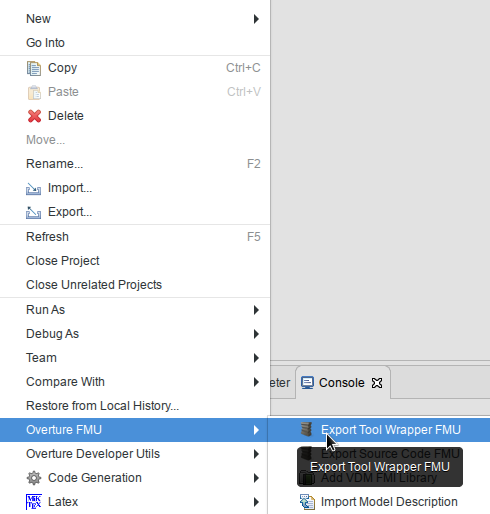
\includegraphics[width=3.5in]{figures/toolWrapperExportOverture.png}
\caption{Exporting a tool-wrapper FMU.}
\label{fig:toolwrapperexportoverture}
\end{figure}
\clearpage
%
%
%
\subsubsection{Standalone FMU Export}
In contrast to tool-wrapper FMUs, models exported as standalone FMUs do not require Overture in order to simulate.
%
Instead, they are first passed through Overture's C code generator such that a standalone implementation of the model is first obtained.
%
Once compiled, this executable model then replaces the combination of VDM interpreter and model, and the FMU executes natively on the co-simulation platform.
%
Currently Mac OS, Windows and Linux are supported.

The export process consists of two steps.
%
First, a source code FMU is obtained from Overture as shown in Figure \ref{fig:standaloneexportoverture}.
%
Second, the \intoapp{} must be used to upload the resulting FMU to the FMU compilation server using the built-in facility described in Section \ref{sub:other-features}.
%
This is accessed by navigating to \emph{Window} $\rightarrow$ \emph{Show FMU Builder}.

Please note that only some features of VDM-RT are currently supported by the C code generator.
%
This is discussed in more detail in Section \ref{sec:CodeGen}.
%
%
%
\begin{figure}[ht]
\centering
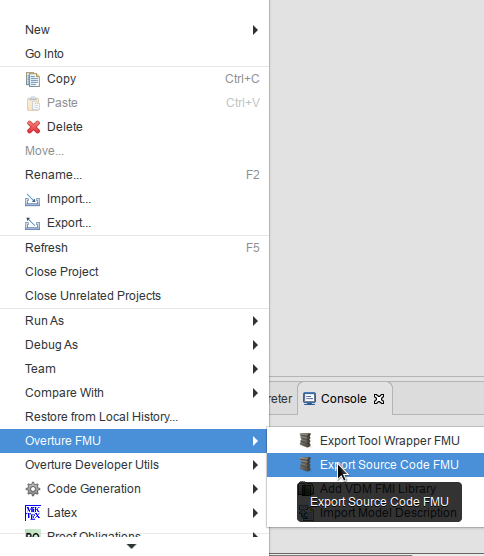
\includegraphics[width=3.5in]{figures/standaloneExportOverture.png}
\caption{Exporting a standalone FMU.}
\label{fig:standaloneexportoverture}
\end{figure}
%
%
%
%\clearpage

%
%
%
\subsection{20-sim}\label{sec:simulators:20sim}
This section explains the FMI and INTO-CPS related features of {20-sim}\footnote{Note that 20-sim is Windows-only. However, it can run fine using Wine \cite{winehq2016} on other platforms. For details on using 20-sim under Wine, contact Controllab.}.
%
We focus on the import of \texttt{model\allowbreak{}Description.\allowbreak{}xml} files, standalone and tool-wrapper FMU export (FMU slave), 3D visualization of FMU operation and an experimental FMU import (FMU master) feature.
%
The complete {20-sim} tool documentation can be found in the {20-sim} Reference Manual \cite{20simReference16a}.

\subsubsection{Import of \texttt{modelDescription.xml} File}\label{sec:simulators:20sim:modeldescriptionimport}
{20-sim} can automatically generate an empty {20-sim} submodel
\footnote{Note that the term ``submodel'' here should not be confused with the INTO-CPS notion of a ``constituent model''.  A submodel here is a part in a graphical 20-sim model.}
from a \texttt{mo\-del\-Description\-.xml} file.
To use the \texttt{modelDescription\allowbreak{}.xml} import, you will need to use the special ``4.6.4-intocps'' version of 20-sim\footnote{You can download the INTO-CPS version of 20-sim using the Download Manager in the INTO-CPS Application.}.
%
A \texttt{mo\-del\-Description\allowbreak{}.xml} file can be imported into {20-sim} by using Windows Explorer to drag the \texttt{model\-Description\allowbreak{}.xml} file onto your {20-sim} model (see \autoref{figure:20-sim_import_modelDescription}).
%
%
%
This creates a new empty submodel with a blue icon that has the same inputs and outputs as defined in the \texttt{modelDescription\allowbreak{}.xml} file.
%
%
%
\begin{figure}[hpt]
	\centerline{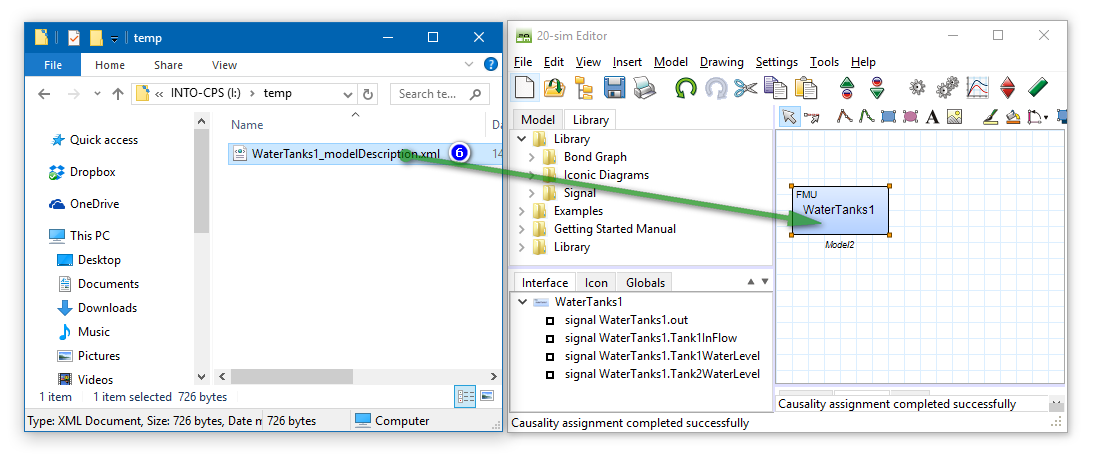
\includegraphics[width=\textwidth]{figures/20-sim_import_modelDescription.png}}
	\caption{Import a Model Description in 20-sim.}
	\label{figure:20-sim_import_modelDescription}
\end{figure}
%
%
%
\subsubsection{Tool-wrapper FMU Export}\label{sec:simulators:20sim:toolwrapperfmu}
A tool-wrapper FMU is a communication FMU that opens the original model in the modelling tool and takes care of remotely executing the co-simulation steps inside the modelling tool using some tool-supported communication mechanism.
%
{20-sim} supports co-simulation using the XML-RPC-based DESTECS co-simulation interface \cite{DESTECSD32b}.
%
The generation of a tool-wrapper FMU involves two steps that will be explained below:
\begin{enumerate}
  \item Extend the model with co-simulation inputs, outputs and shared design parameters.
  \item Generate a model-specific tool-wrapper FMU.
\end{enumerate}

The tool-wrapper approach involves communication between the co-si\-mu\-la\-tion engine (COE) and the {20-sim} model through the tool-wrapper FMU.
The {20-sim} model should be extended with certain variables that can be set or read by the COE.
These variables are the co-simulation inputs and outputs.
They can be defined in the model in an equation section called \texttt{externals}:  

\begin{lstlisting}
externals
	real global export mycosimOutput;
	real global import mycosimInput;
\end{lstlisting}

To make it possible to set or read a parameter by the co-simulation engine, it should be marked as \texttt{'shared'}:

\begin{lstlisting}
parameters
	// shared design parameters
	real mycosimParameter ('shared') = 1.0;
\end{lstlisting}

The next step is to generate a tool-wrapper FMU for the prepared model.
This requires at least the ``{4.6.3}-intocps'' version of {20-sim}\footnote{You can download the INTO-CPS version of 20-sim using the Download Manager in the INTO-CPS Application.}.
This version of {20-sim} comes with a Python script that generates a tool-wrapper FMU for the loaded model.

To generate the tool-wrapper FMU:
\begin{enumerate}
  \item Make sure that the tool-wrapper prepared {20-sim} model is saved at a writable location.
  The tool-wrapper FMU will be generated in the same folder as the model.
  \item Open the prepared {20-sim} model in {20-sim}.
  \item In the 20-sim Editor window, open the menu \textit{Tools} and select the menu option \textit{Generate Toolwrapper FMU}.
  \item You can find the generated tool-wrapper FMU as \textit{<modelname>.fmu} in the same folder as your model.

\end{enumerate}

%
%
%
\subsubsection{Standalone FMU Export}\label{sec:simulators:20sim:standalonefmu}
Starting with {20-sim} version 4.6, the tool has a built-in option to generate standalone co-simulation FMUs for both FMI 1.0 and 2.0.

To export a {20-sim} submodel as a standalone FMU, make sure that the part of the model that you want to export as an FMU is contained in a submodel and simulate your model to confirm that it behaves as desired.

Next, follow these steps (see also \autoref{figure:20sim_export_fmu}):
%
%
%
\begin{figure}[hbt]
	\centerline{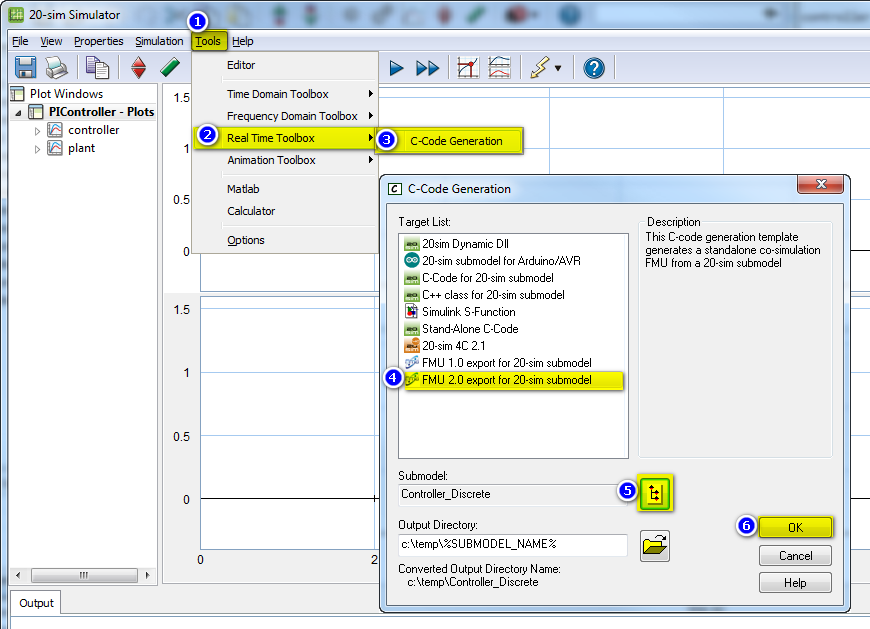
\includegraphics[width=\textwidth]{figures/20-sim_generate_fmu.png}}
	\caption{Export an FMU from 20-sim.}
	\label{figure:20sim_export_fmu}
\end{figure}
%
%
%
\begin{enumerate}
  \item In the Simulator window, choose from the menu: \textit{Tools}.
  \item Select \textit{Real Time Toolbox}.
  \item Click \textit{C-Code Generation}.
  \item Select the \textit{FMU 2.0 export for 20-sim submodel} target. 
  \item Select the submodel to export as an FMU.
  \item Click OK to generate the FMU. This will pop-up a blue window.
\end{enumerate}
%
%
%
Note that to automatically compile the FMU, you will need the Microsoft Visual C++ 2010, 2013 or 2015 compiler installed (normally included with Microsoft Visual Studio, either Express or Community edition).
%
If {20-sim} can find one of the supported VC++ compilers, it starts the compilation and reports where you can find the newly generated FMU.
%
The {20-sim} FMU export also generates a \textit{Makefile} that allows you to compile the FMU on Windows using Cygwin, MinGW, MinGW64 or on Linux or MacOS X.\\
%
{20-sim} can currently export only a subset of the supported modelling language elements as standalone C-code.
%
Full support for all {20-sim} features is only possible through the tool-wrapper FMU approach (described shortly in Section \ref{sec:simulators:20sim:toolwrapperfmu}).
%
The original goal for the {20-sim} code generator was to export control systems into ANSI-C code to run the control system under a real-time operating system.
%
As a consequence, {20-sim} currently only allows code generation for discrete-time submodels or continuous-time submodels using a fixed-step integration method.
%
Support for variable step size integration methods is not yet included by default in the official {20-sim} 4.6 release, but it is already included in the {20-sim} ``4.6.2-intocps'' release and on GitHub (see below).
%
Other language features that are not supported, (or are only partly supported) for code generation, are:
%
%
%
\begin{itemize}
\item \textbf{Hybrid models:} Models that contain both discrete-\@ and continuous-time sections cannot be generated at once. However, it is possible to export the continuous and discrete blocks separate.
\item \textbf{File I/O:} The 20-sim ``{Table2D}'' block is supported; the ``datafromfile'' block is not yet supported.
\item \textbf{External code:} Calls to external code are not supported. Examples are: \texttt{DLL()}, \texttt{DLLDynamic()} and the MATLAB functions.
\item \textbf{Variable delays:} The \texttt{tdelay()} function is not supported due to the requirement for dynamic memory allocation.
\item \textbf{Event functions:} \texttt{timeevent()}, \texttt{frequencyevent()} statements are ignored in the generated code.
\item \textbf{Fixed-step integration methods:} \textit{Euler}, \textit{Runge-Kutta 2} and \textit{Runge-Kutta 4} are supported.
\item \textbf{Implicit models:} Models that contain unsolved algebraic loops are not supported.
\item \textbf{Variable-step integration methods:} \textit{Vode-Adams} and \textit{Modified Backward Differential Formula} (MeBDF) are available on GitHub (see below for the link).
\end{itemize}

The FMU export feature of {20-sim} is being improved continuously based on feedback from INTO-CPS members and other customers. 
%
To benefit from bug fixes and to try the latest FMU export features like variable step size integration methods (\emph{e.\@g.\@} Vode-Adams and MeBDF), you can download the latest version of the {20-sim} FMU export template from:
%
%
%
\begin{quote}
  \url{https://github.com/controllab/fmi-export-20sim}
\end{quote}
%
%
%
Detailed instructions for the installation of the GitHub version of the {20-sim} FMU export template can be found on this GitHub page.
The GitHub FMU export template can be installed alongside the existing built-in FMU export template.
%
%
%

\subsubsection{FMI 2.0 Import}\label{sec:simulators:20sim:fmuimport}
The ``{4.6.4}-intocps'' version of {20-sim} has an experimental option to import an FMU directly in {20-sim} for co-simulation within {20-sim} itself.
This is useful for quickly testing exported FMUs without the need to set-up a full co-simulation experiment in the INTO-CPS application.
Presently it can only import FMI 1.0 and 2.0 \textit{co-simulation} FMUs can be imported.

The procedure for importing an FMU as {20-sim} submodel is similar to importing a \texttt{modelDescription\allowbreak{}.xml} file.
Follow these steps to import an FMU in {20-sim}:
%
%
%
\begin{enumerate}
  \item Copy/move the FMU to the same folder as your model. This is not required but recommended to prevent embedding hardcoded paths in your model.
  \item Using Windows Explorer, drag the FMU file on your {20-sim} model (see \autoref{figure:20-sim_import_fmu}). 
\end{enumerate}
%
%
%
\begin{figure}[ht]
	\centerline{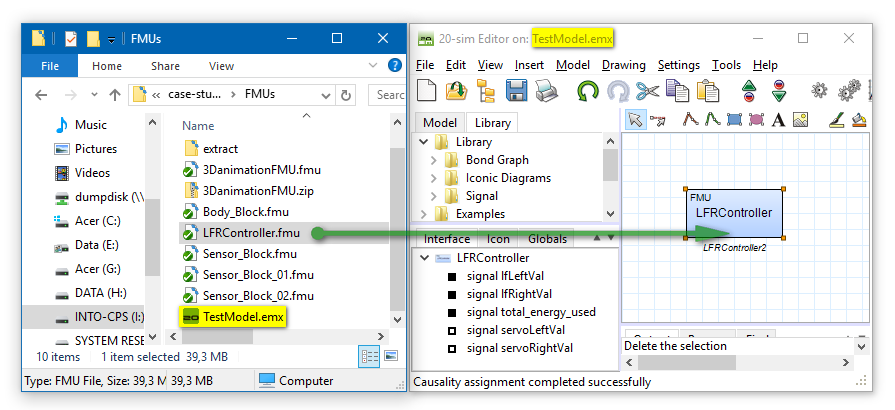
\includegraphics[width=\textwidth]{figures/20-sim_import_fmu.png}}
	\caption{Importing an FMU in 20-sim.}
	\label{figure:20-sim_import_fmu}
\end{figure}
%
%
%
This creates a new submodel with a blue icon that acts as an FMU wrapper. FMU inputs and outputs are translated into {20-sim} submodel input and output signals.
FMU parameters (scalar variables with causality ``parameter'') are also available in {20-sim}.
This means that you can alter the default values of these FMU parameters in {20-sim}.
The altered FMU parameters are transferred to the FMU during the initialization mode phase of the FMU.


%
%
%
\subsection{20-sim 4C}\label{sec:simulators:20sim4C}
This section describes the features of {20-sim 4C} \cite{20sim4C} \footnote{Note that 20-sim 4C is Windows-only, but it can be executed using Wine \cite{winehq2016} on other platforms.} developed specifically in support of INTO-CPS and FMI.
%
{20-sim 4C} is a rapid prototyping tool that facilitates running C code on hardware to control machines and systems.
%
{20-sim 4C} imports models (as generated C code) from multiple sources (\emph{e.\@g.\@} 20-sim) and runs them on hardware targets such as embedded ARM boards (\emph{e.\@g.\@} Raspberry Pi), PCs running real-time Linux and industrial PLCs.

One of the goals of the \into project is to extend the capabilities of the \into tool chain toward executing part of a co-simulation on real hardware in real-time.
%
This is known as Hardware-in-the-Loop (HiL) simulation.
%
This section explains how the FMI import and export features of {20-sim 4C} can be used to execute source code FMUs on hardware targets in co-simulation under the control of the COE.
%
The complete {20-sim} tool documentation can be found in the {20-sim 4C} Reference Manual \cite{20sim4CManual13a}.
%
All details of the implementation of FMI support in 20-sim 4C can be found in Deliverable D4.3b \cite{INTOCPSD4.3b}.
%
%
%
\subsubsection{Source Code FMU Import}\label{sec:simulators:20sim4C:fmuimport}
To import an FMU in {20-sim 4C}, it must first be converted to a valid {20-sim 4C} project.
%
This is currently done via a command line call at the Windows Command prompt.
%
The command to import a source code FMU in {20-sim 4C} is:
%
%
%
\begin{quote}
\texttt{C:\textbackslash{}Program Files (x86)\textbackslash{}20-sim 4C 2.2\textbackslash{}bin\textbackslash{}\\20simparser.exe newfmuProjectName fmuFilename.fmu}\\
\end{quote}
%
%
%
where \texttt{newfmuProjectName} is the name of a new directory in which {20-sim 4C} will generate the new project.
%
This directory is created as a subdirectory of the current directory.
%
An example is shown in \autoref{figure:20-sim-4C_fmu_import1}.
%
%
%
\begin{figure}[hpt]
	\centerline{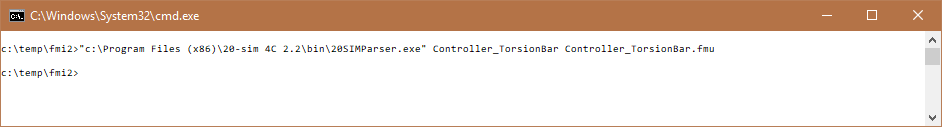
\includegraphics[width=\textwidth]{figures/20-sim-4C_fmu_import1.png}}
	\caption{Import a source code FMU in 20-sim 4C.}
	\label{figure:20-sim-4C_fmu_import1}
\end{figure}
%
%
%
This example creates a new directory in \texttt{C:\textbackslash{}Temp\textbackslash{}fmi2} named \texttt{Controller\_TorsionBar} and briefly shows the import dialog from \autoref{figure:20-sim-4C_fmu_import2}.
%
%
%
\begin{figure}[hpt]
	\centerline{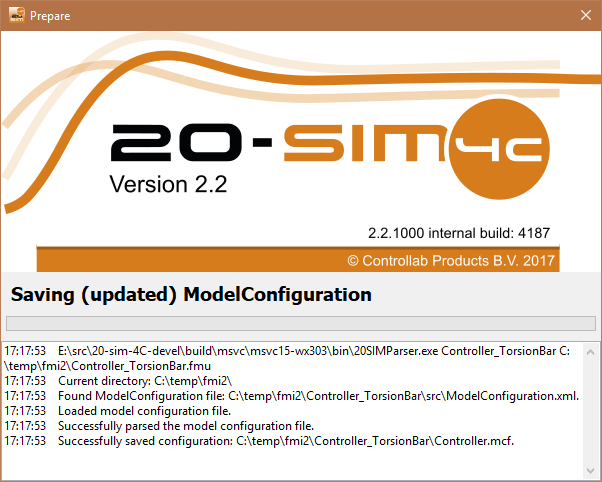
\includegraphics[width=0.8\textwidth]{figures/20-sim-4C_fmu_import2.png}}
	\caption{20-sim 4C FMU importer.}
	\label{figure:20-sim-4C_fmu_import2}
\end{figure}
%
%
%
After successfully extracting and importing the FMU, 20-sim 4C will start.

Source code FMUs are deployed to a real-time target as follows:
%
%
%
\begin{enumerate}
\item The 20-sim 4C window (\autoref{figure:20-sim-4C_select_target}) shows the name of the FMU and its public variables and parameters in the tree at the left side.
% 
\begin{figure}[hpt]
	\centerline{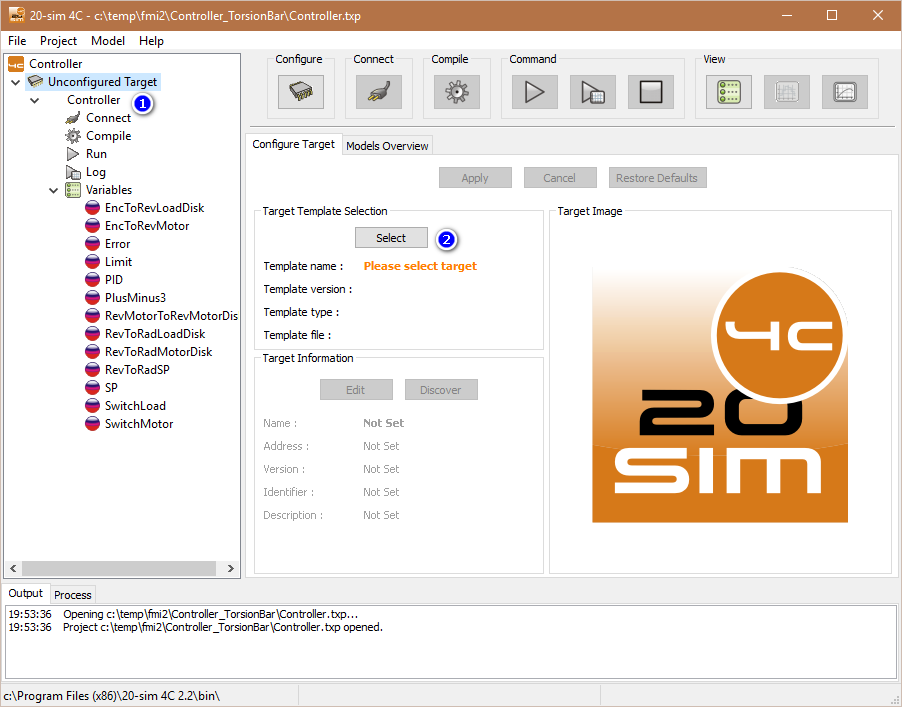
\includegraphics[width=\textwidth]{figures/20-sim-4C_select_target.png}}
	\caption{20-sim 4C project with imported FMU.}
	\label{figure:20-sim-4C_select_target}
\end{figure}
%
\item Use the \textit{Select} button in the \textit{Target Template Selection} box to select the hardware target for the FMU.  This shows the \textit{Select Target Configuration} dialog (\autoref{figure:20-sim-4C_select_raspberry_pi}.)
%
\begin{figure}[hpt]
	\centerline{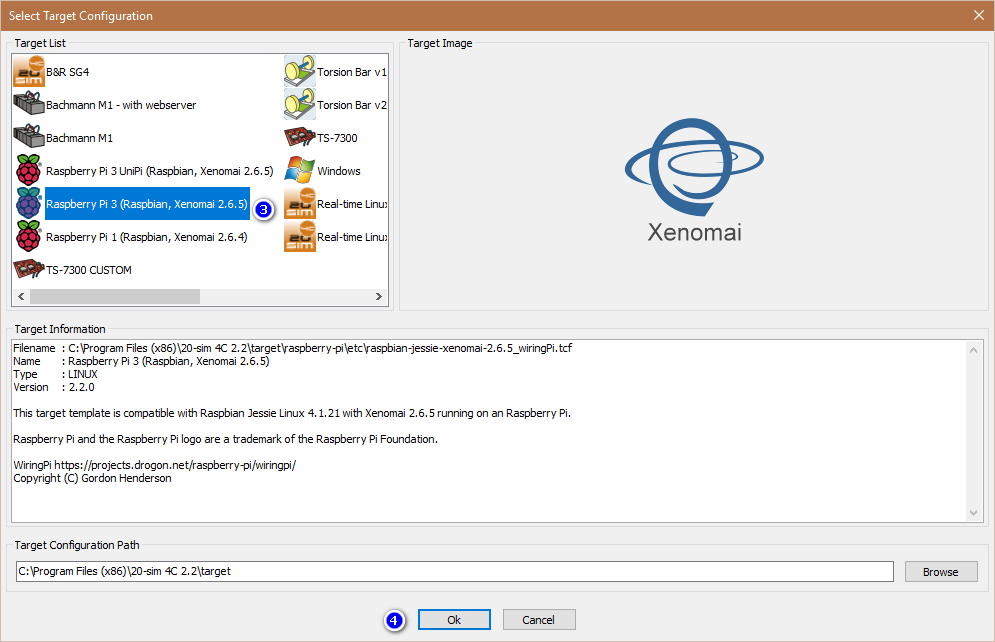
\includegraphics[width=\textwidth]{figures/20-sim-4C_select_raspberry_pi.png}}
	\caption{Select the Raspberry Pi target.}
	\label{figure:20-sim-4C_select_raspberry_pi}
\end{figure}
%
\item Select the \textit{Raspberry Pi 3 (Raspbian, Xenomai 2.6.5)} target.
\item Press the \textit{OK} button to confirm. This will automatically trigger a network scan to find the Raspberry Pi on the network.
\item In case multiple targets are found, select the desired target in the \textit{Please select a target} dialog (\autoref{figure:20-sim-4C_select_multiple_targets}) and press \textit{OK}.
%
%
%
\begin{figure}[hpt]
	\centerline{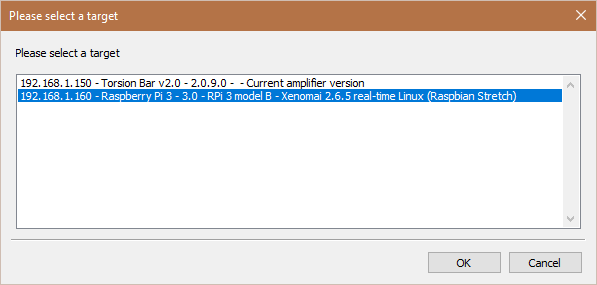
\includegraphics[width=0.8\textwidth]{figures/20-sim-4C_select_multiple_targets.png}}
	\caption{Select the right target.}
	\label{figure:20-sim-4C_select_multiple_targets}
\end{figure}
%
\item In the main 20-sim 4C window, press \textit{Apply} to confirm the target settings.  20-sim 4C will now try to connect to the Raspberry Pi. When the connection is successful, the \textit{Configure} button will turn green.
  See \autoref{figure:20-sim-4C_connect}.
%
\begin{figure}[hpt]
	\centerline{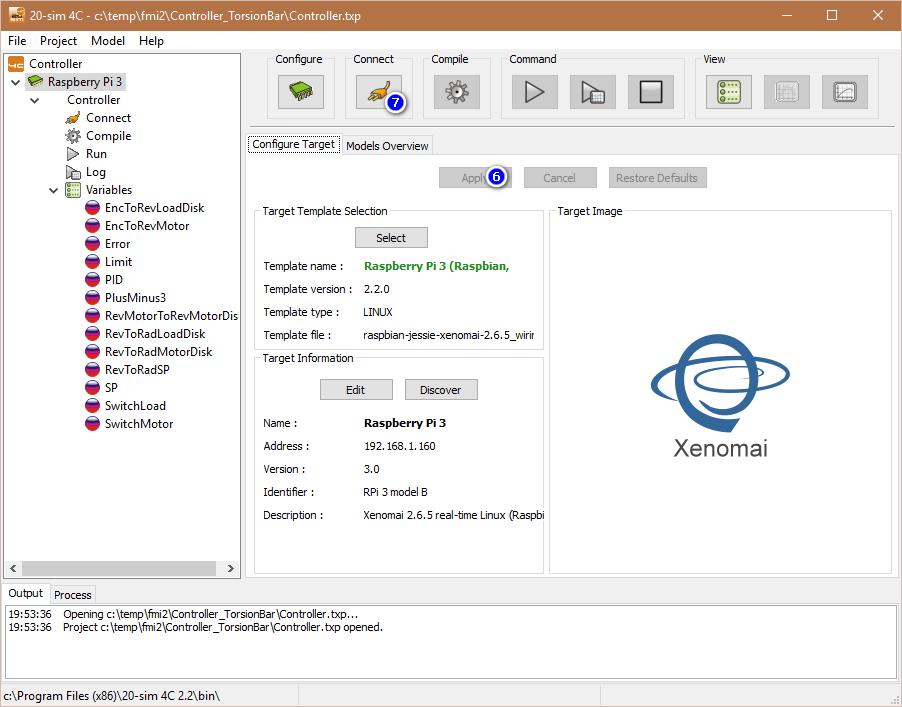
\includegraphics[width=\textwidth]{figures/20-sim-4C_connect.png}}
	\caption{Accept target settings and go to the connection phase.}
	\label{figure:20-sim-4C_connect}
\end{figure}
%
\item Click the \textit{Connect} button to go to the connection phase. This will show the inputs and outputs of the FMU and 20-sim 4C allows you to connect them to the on-board I/O pins.
%
\item To connect an input or output,  select the signal and press the \textit{Connect} button or double-click the signal (\autoref{figure:20-sim-4C_connect_io}.)  This will show the \textit{Connection} dialog as shown in \autoref{figure:20-sim-4C_connect_select_component}.
%
\begin{figure}[hpt]
	\centerline{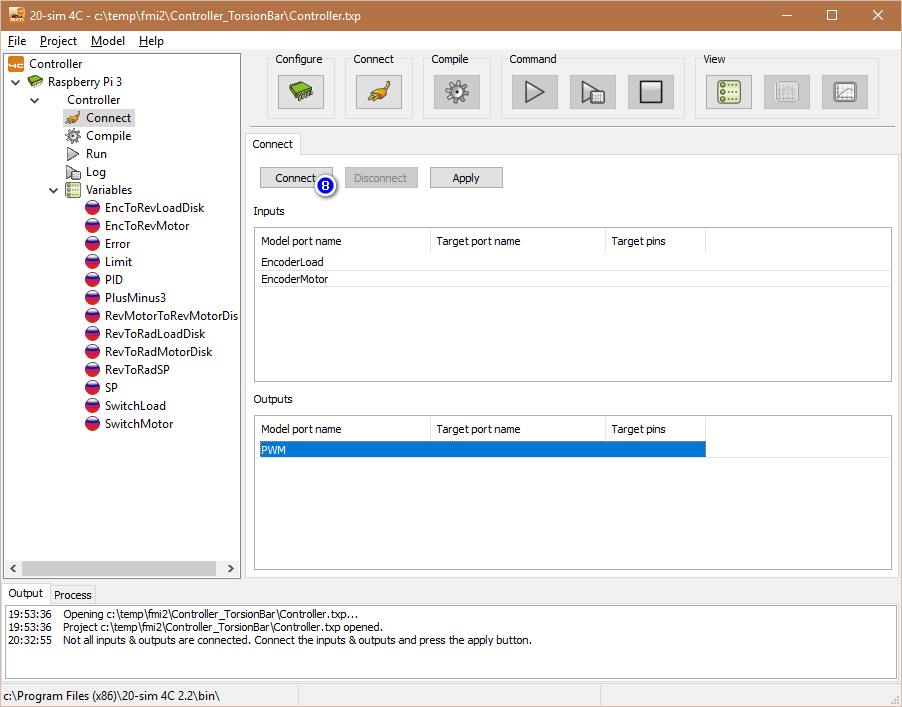
\includegraphics[width=\textwidth]{figures/20-sim-4C_connect_io.png}}
	\caption{Select an input or output and press \emph{Connect}.}
	\label{figure:20-sim-4C_connect_io}
\end{figure}
%
\item The connection dialog allows you to select an I/O component (\emph{e.\@g.\@} GPIO for digital I/O or PWM; see \autoref{figure:20-sim-4C_connect_select_component}) and a port within this component (typically a physical pin or connector on the target device; see \autoref{figure:20-sim-4C_connect_select_port}).  Select \textit{OK} to confirm the connection.  The I/O available depends on the selected target device.  The Raspberry Pi 3 provides by default only digital inputs and outputs and 2 PWM outputs.  Extension boards are needed for other I/O.\\
  \textbf{\textit{Note:}}  In case you would like to use an extension board or external I2C or SPI based I/O chip or other I/O, feel free to ask Controllab for options to support this in 20-sim 4C.
%
\begin{figure}[hpt]
	\centerline{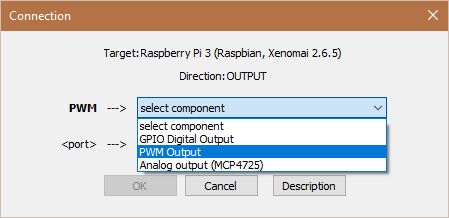
\includegraphics[width=0.6\textwidth]{figures/20-sim-4C_connect_select_component.png}}
	\caption{Select a component.}
	\label{figure:20-sim-4C_connect_select_component}
\end{figure}
%
\begin{figure}[hpt]
	\centerline{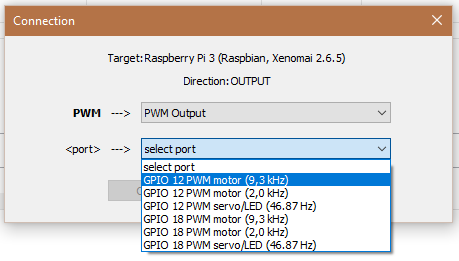
\includegraphics[width=0.6\textwidth]{figures/20-sim-4C_connect_select_port.png}}
	\caption{Select a port.}
	\label{figure:20-sim-4C_connect_select_port}
\end{figure}
%
\item When you have connected all desired inputs and outputs to the I/O, press the \textit{Apply} button (\autoref{figure:20-sim-4C_connect_apply}.)  The \textit{Connect} button will turn green and 20-sim 4C will extend the FMU source code with additional files to provide support for the Raspberry Pi Xenomai real-time Linux and the Raspberry Pi I/O.\\
%
\textbf{\textit{Note:}} It is not required to connect all inputs and outputs to real I/O.  20-sim 4C will show a warning when some inputs or outputs are not connected.  Unconnected inputs will read a zero (0) value by default.  A special real-time toolwrapper FMU can be generated from 20-sim 4C that will allow you to write to unconnected inputs from a co-simulation experiment (see section \ref{sec:simulators:20sim4C:fmuexport}).  This toolwrapper FMU will also allow you to read all FMU exported variables including all inputs and outputs even when inputs and outputs are connected to the I/O.  This toolwrapper FMU is the basis for INTO-CPS HiL simulation with the Raspberry Pi as the real-time target.
%
\begin{figure}[hpt]
	\centerline{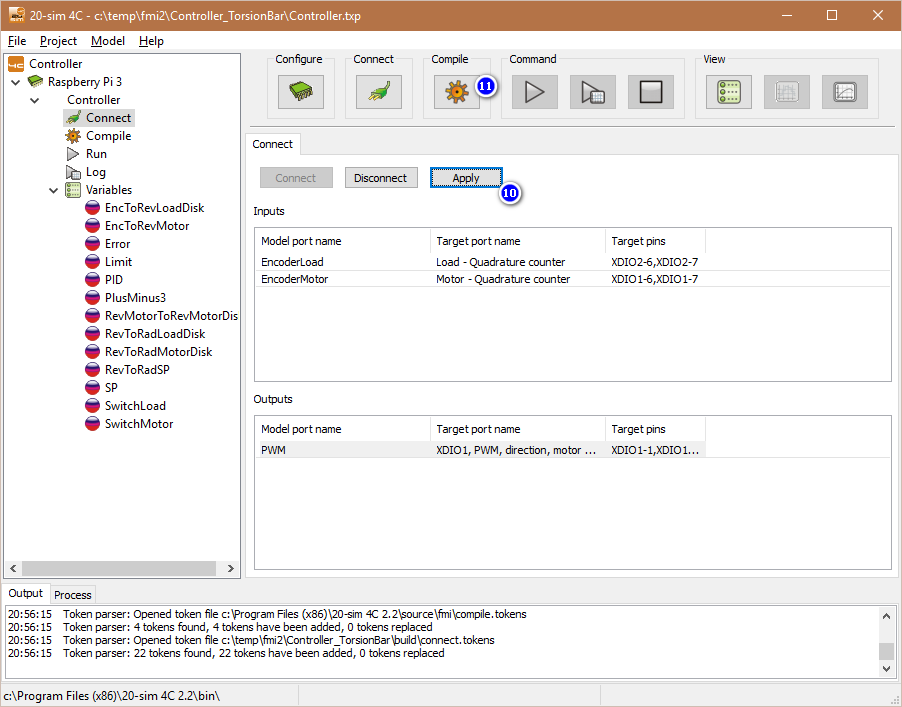
\includegraphics[width=\textwidth]{figures/20-sim-4C_connect_apply.png}}
	\caption{Apply the connections and compile the code.}
	\label{figure:20-sim-4C_connect_apply}
\end{figure}
%
\item Press the orange \textit{Compile} button (\autoref{figure:20-sim-4C_connect_apply}) to go to the \textit{Compile} phase.  This will compile the FMU source code and the additional 20-sim 4C source code into a real-time application.
%
\item When the compilation process is ready and successful, click the orange \textit{Command} button to configure the last task settings before uploading the compiled FMU to the Raspberry Pi (\autoref{figure:20-sim-4C_compile}.)
%
\begin{figure}[hpt]
	\centerline{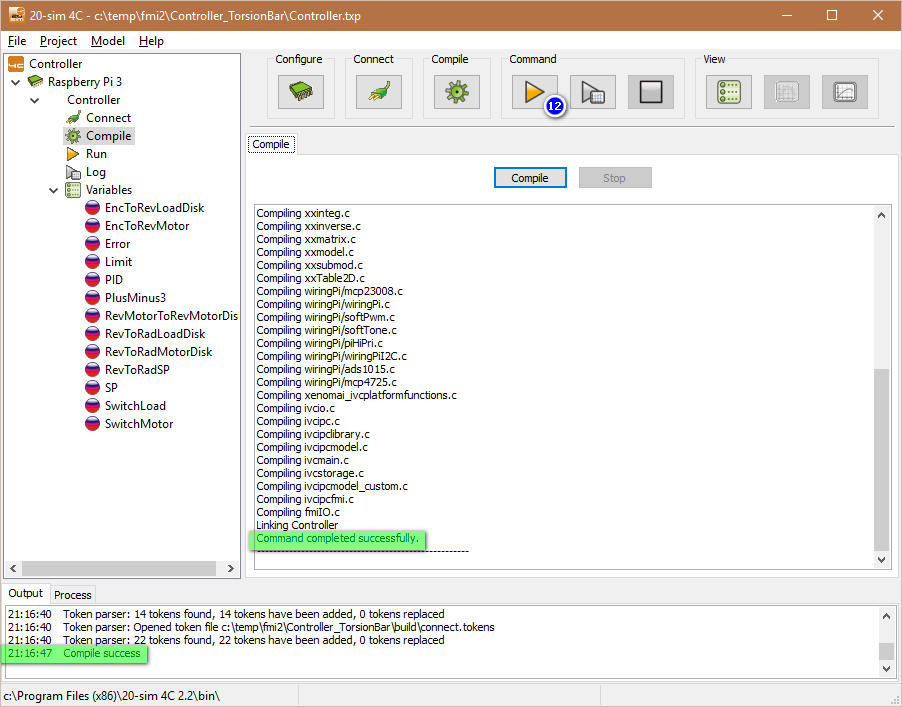
\includegraphics[width=\textwidth]{figures/20-sim-4C_compile.png}}
	\caption{Compilation phase.}
	\label{figure:20-sim-4C_compile}
\end{figure}
%
\item On the \textit{Configure Run} tab (\autoref{figure:20-sim-4C_run_settings}), you can specify the finish time of the FMU or disable it if it should run forever (until reboot/shutdown).  Ensure that the \textit{Discrete Time Interval} has a step size larger than 0.  This value is used as the time (step size) between two FMU ``doStep'' calls and determines the FMU calculation frequency.  The Raspberry Pi 3 is able to support step sizes as low as 0.00005 (20 kHz), but this depends on the FMU computation load and number of connected I/O pins.
%
\begin{figure}[hpt]
	\centerline{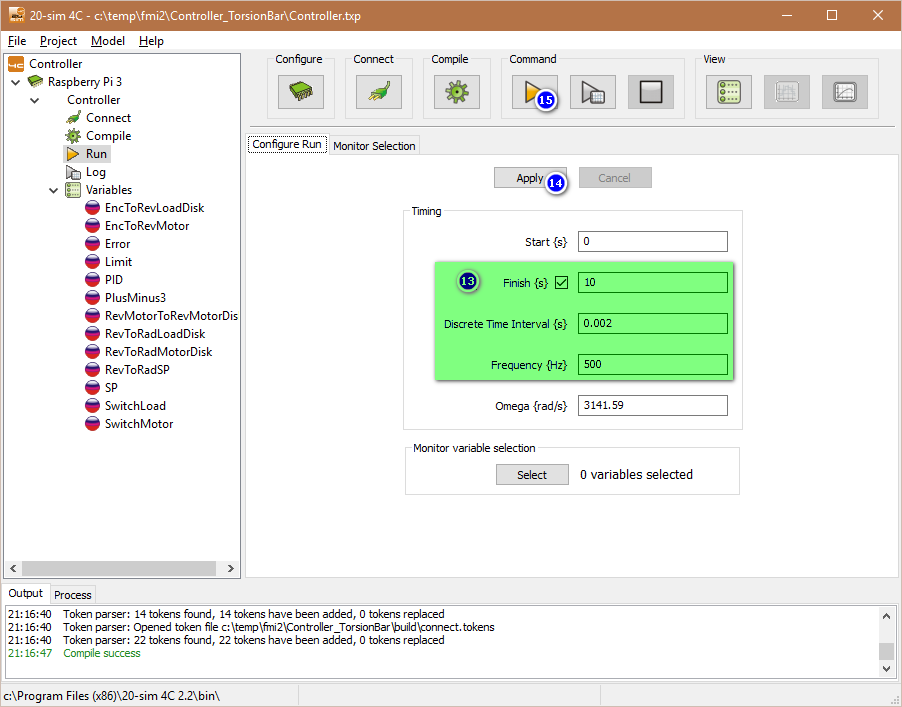
\includegraphics[width=\textwidth]{figures/20-sim-4C_run_settings.png}}
	\caption{Configure task run settings.}
	\label{figure:20-sim-4C_run_settings}
\end{figure}
%
\item Press the \textit{Apply} button to store the run settings.  The \textit{Command} button will turn green.
%
\item Click the \textit{Command} button to upload and start your FMU on the Raspberry Pi.  If everything is configured correctly, the FMU will start and 20-sim 4C will monitor its progress and the current value of the FMU variables.
%
\begin{figure}[hpt]
	\centerline{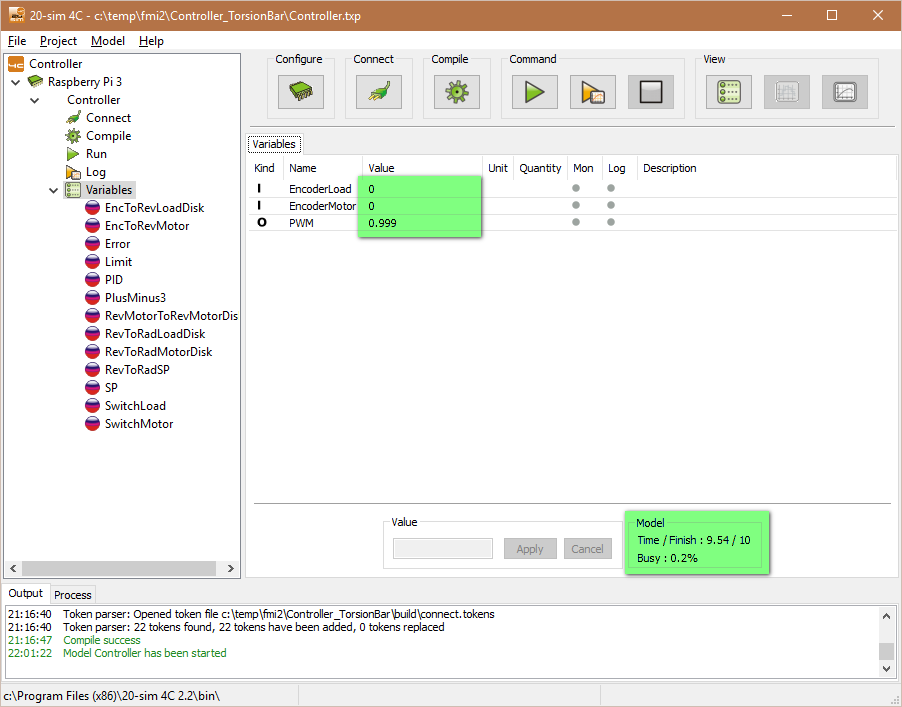
\includegraphics[width=\textwidth]{figures/20-sim-4C_running.png}}
	\caption{FMU is running.}
	\label{figure:20-sim-4C_running}
\end{figure}
%
\item It is also possible to show selected variables in a monitor plot.  You can enable monitoring of a signal by toggling the dot icon in the \textit{Mon} column to a monitor icon.
%
\item Click the large monitor icon on the button bar to show the monitor plot. An example of the monitor plot with three I/O signals is shown in \autoref{figure:20-sim-4C_monitoring_plot}.
%
\begin{figure}[hpt]
	\centerline{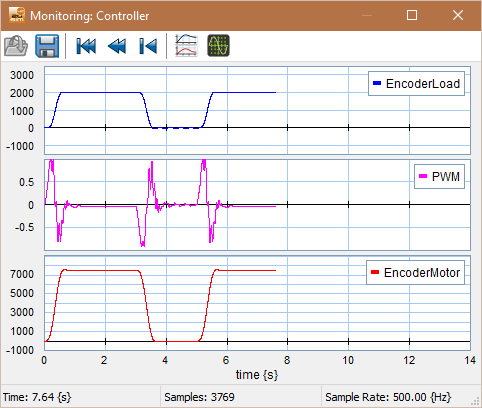
\includegraphics[width=0.7\textwidth]{figures/20-sim-4C_monitoring_plot.png}}
	\caption{Variable monitor.}
	\label{figure:20-sim-4C_monitoring_plot}
\end{figure}  
%  
\end{enumerate}
%
%
%
\subsubsection{Real-time toolwrapper FMU export}\label{sec:simulators:20sim4C:fmuexport}
For HiL simulation with a Raspberry Pi, 20-sim 4C is extended with FMU export functionality.
%
The 20-sim 4C FMU export option generates a real-time toolwrapper FMU for the currently loaded 20-sim 4C project.
%
This FMU can be used in the COE to interface the real-time FMU running on the Raspberry Pi with a standard COE co-simulation experment. 
%
Assuming a running application on the Raspberry Pi, FMU export can be performed as follows:
%
%
%
\begin{enumerate}
\item Co-simulation using a toolwrapper FMU uses the unconnected 20-sim 4C inputs.  Make sure that the desired co-simulation inputs are not connected during the 20-sim 4C \textit{Connect} phase (\autoref{figure:20-sim-4C_connect_apply}).
%
\item Export an FMU using the \textit{FMU Export} menu item.  Make sure that the ``Raspberry Pi 3'' target, or the 20-sim 4C  project (your FMU name,) is selected in the left tree.  This is required so that the FMU exporter can find the right 20-sim 4C project.
%
\item Select \textit{Export FMU} from the \textit{Project} menu item. See \autoref{figure:20-sim-4C_export_toolwrapper_fmu}.
% 
\begin{figure}[hpt]
	\centerline{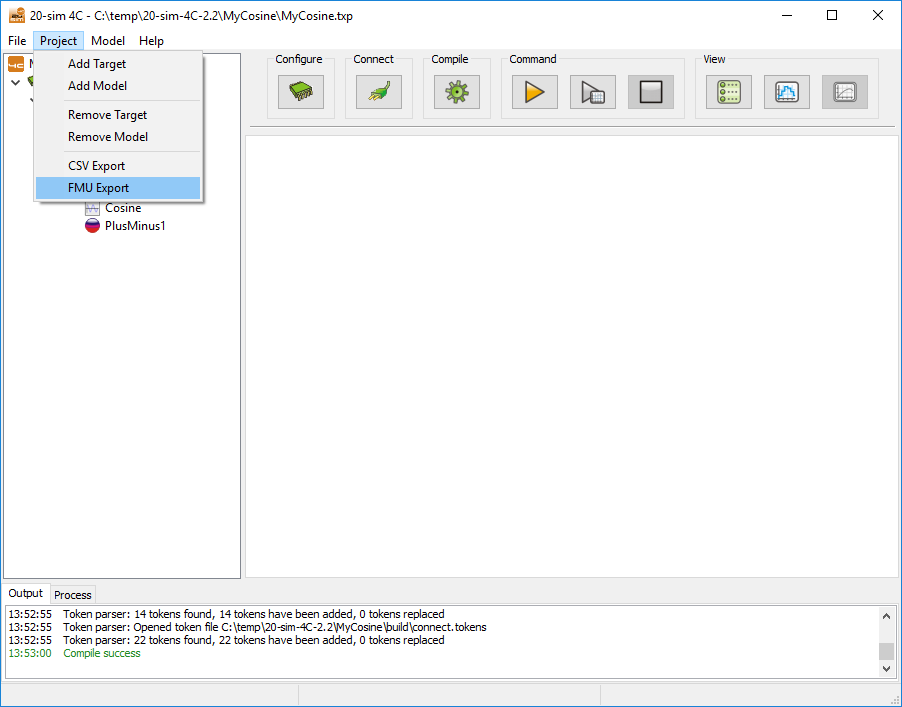
\includegraphics[width=\textwidth]{figures/20-sim-4C_export_toolwrapper_fmu.png}}
	\caption{Export toolwrapper FMU.}
	\label{figure:20-sim-4C_export_toolwrapper_fmu}
\end{figure}
%
\item A command-line window will be displayed showing status information of the FMU toolwrapper creation process.  See \autoref{figure:20-sim-4C_export_toolwrapper_fmu2}.
%
\begin{figure}[hpt]
	\centerline{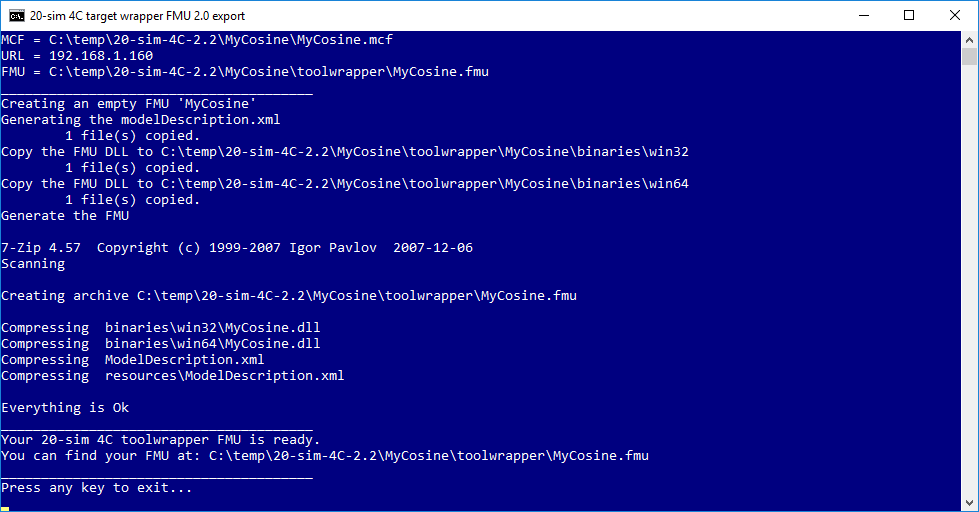
\includegraphics[width=\textwidth]{figures/20-sim-4C_export_toolwrapper_fmu2.png}}
	\caption{Toolwrapper FMU status.}
	\label{figure:20-sim-4C_export_toolwrapper_fmu2}
\end{figure}
%
\item This window can be closed after noting the location of the generated FMU.
%
\item The newly created FMU can be used in 32-bit and 64-bit Windows FMI co-simulators like the INTO-CPS COE.  Linux and MacOS X compatible versions are not yet available.
\end{enumerate}

%
%
%
\subsection{OpenModelica}
This section explains the FMI and INTO-CPS related features of OpenModelica.
%
The focus is on import of \texttt{model\allowbreak{}Description.\allowbreak{}xml} files and standalone and tool-wrapper FMU export.
%
%
%
\subsubsection{Import of \texttt{modelDescription.xml} Files}\label{sec:simulators:openmodelica:modeldescriptionimport}
OpenModelica can import \texttt{modelDescription\allowbreak{}.xml} interface files created using Modelio and create Modelica models from them.
%
To use the \texttt{modelDescription\allowbreak{}.xml} import feature, you will need to use OpenModelica nightly-builds versions, as this extension is new.
%
Nightly builds can be obtained through the main INTO-CPS GitHub site:
%
%
%
\begin{quote}
\url{http://into-cps-association.github.io}
\end{quote}
%
%
%

To import a \texttt{modelDescription\allowbreak{}.xml} file in OpenModelica one can use:
\begin{enumerate}
\item The OpenModelica Connection Editor GUI (OMEdit): \emph{FMI} $\rightarrow$ \emph{Import FMI Model Description}.
\item A MOS script, \emph{i.\@e.\@} \texttt{script.mos}, see below.
\end{enumerate}
%
%
%
\begin{lstlisting}[language=modelica]
// start script.mos
// import the FMU modelDescription.xml
importFMUModeldescription("path/to/modelDescription.xml"); getErrorString();
// end script.mos
\end{lstlisting}
%
%
The MOS script can be executed from command line via:
\begin{lstlisting}
// on Linux and Mac OS
> path/to/omc script.mos
// on Windows
> %OPENMODELICAHOME%\bin\omc script.mos
\end{lstlisting}

%
The result is a generated file with a Modelica model containing the inputs and outputs specified in \texttt{modelDescription\allowbreak{}.xml}.  For instance:
%
%
%
\begin{lstlisting}[language=modelica]
model Modelica_Blocks_Math_Gain_cs_FMU "Output the product of a gain value with the input signal"
  Modelica.Blocks.Interfaces.RealInput u  "Input signal connector" annotation(Placement(transformation(extent={{-120,60},{-100,80}})));
  Modelica.Blocks.Interfaces.RealOutput y  "Output signal connector" annotation(Placement(transformation(extent={{100,60},{120,80}})));
end Modelica_Blocks_Math_Gain_cs_FMU;"
\end{lstlisting}
%
%
%
%This functionality will ultimately be integrated in the OMEdit (the OpenModelica Connection Editor) graphical user interface.
%
%
%
\subsubsection{FMU Export}
All FMUs exported from OpenModelica are standalone. There are two ways to export an FMU:
%
%
%
\begin{enumerate}
\item From a command prompt.
\item From OMEdit (OpenModelica Connection Editor).
\end{enumerate}
%
%
%
\paragraph{FMU export from a command prompt}
%
To export an FMU for co-simulation from a Modelica model, a Modelica script file \texttt{generateFMU.mos} containing the following calls to the OMC compiler can be used:
%
%
%
\begin{lstlisting}[language=modelica]
// load Modelica library
loadModel(Modelica); getErrorString();

// load other libraries if needed
// loadModel(OtherLibrary); getErrorString();

// generate the FMU: PathTo.MyModel.fmu
translateModelFMU(PathTo.MyModel, "2.0", "cs"); getErrorString();
\end{lstlisting}
%
%
%
Next, the OMC compiler must be invoked on the \texttt{generateFMU\allowbreak{}.mos} script:
%
%
\begin{lstlisting}
// on Linux and Mac OS
> path/to/omc generateFMU.mos
// on Windows
> %OPENMODELICAHOME%\bin\omc generateFMU.mos
\end{lstlisting}
%
%
%
\paragraph{FMU export from OMEdit}
One can also use OMEdit to export an FMU, as detailed in the figures below.
%
%
%
\begin{itemize}
\item Open OMEdit (see \autoref{figure:OMEdit_1}.)
\item Load the model in OMEdit (see \autoref{figure:OMEdit_2}.)
\item Open the model in OMEdit (see \autoref{figure:OMEdit_3}.)
\item Use the menu to export the FMU (see \autoref{figure:OMEdit_4}.)
\item The FMU is now generated (see \autoref{figure:OMEdit_5}.)
\end{itemize}
%
%
%
\begin{figure}[ht]
	\centerline{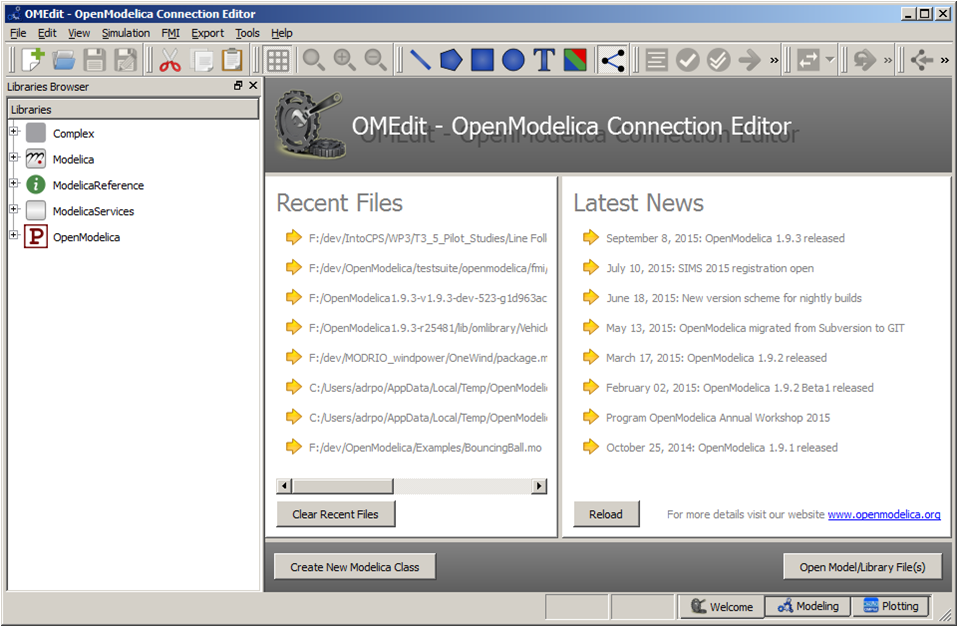
\includegraphics[width=12.5cm]{figures/OMEdit_1.png}}
	\caption{Opening OMEdit.}
	\label{figure:OMEdit_1}
\end{figure}
%
%
%
\begin{figure}[ht]
	\centerline{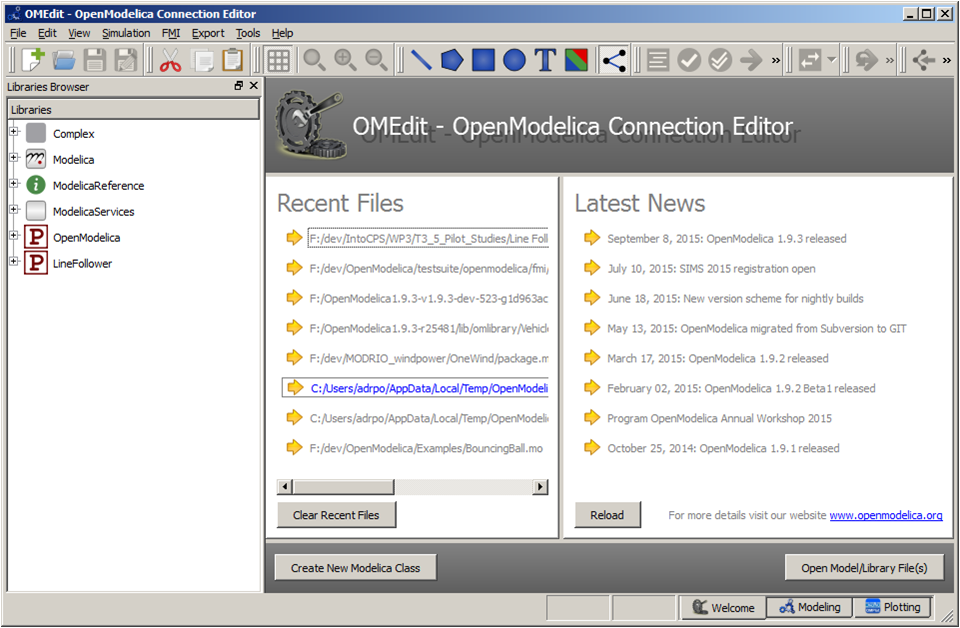
\includegraphics[width=12.5cm]{figures/OMEdit_2.png}}
	\caption{Loading the Modelica model in OMEdit.}
	\label{figure:OMEdit_2}
\end{figure}
%
%
%
\begin{figure}[ht]
	\centerline{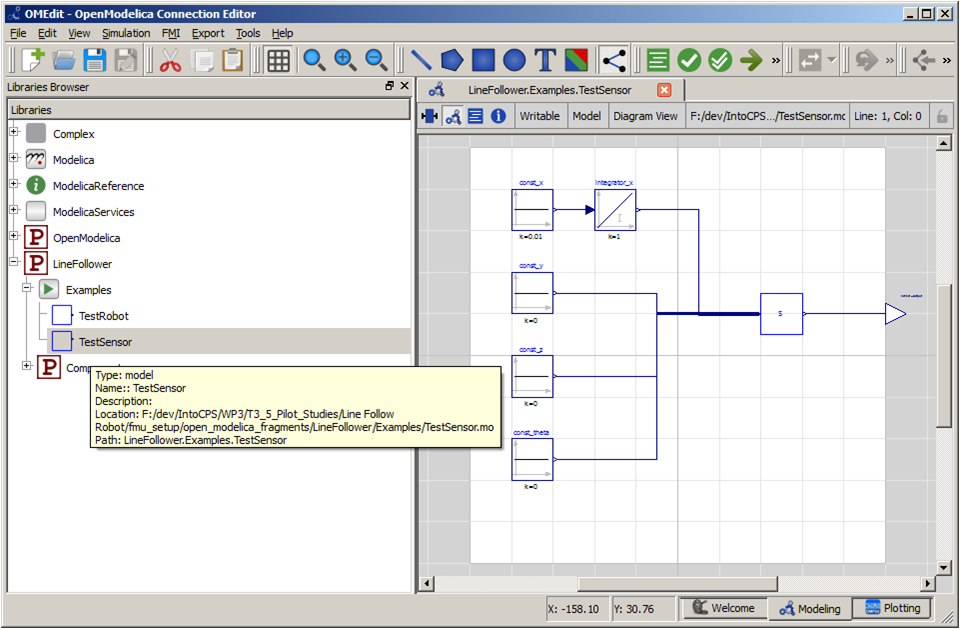
\includegraphics[width=12.5cm]{figures/OMEdit_3.png}}
	\caption{Opening the Modelica model in OMEdit.}
	\label{figure:OMEdit_3}
\end{figure}
%
%
%
\begin{figure}[ht]
	\centerline{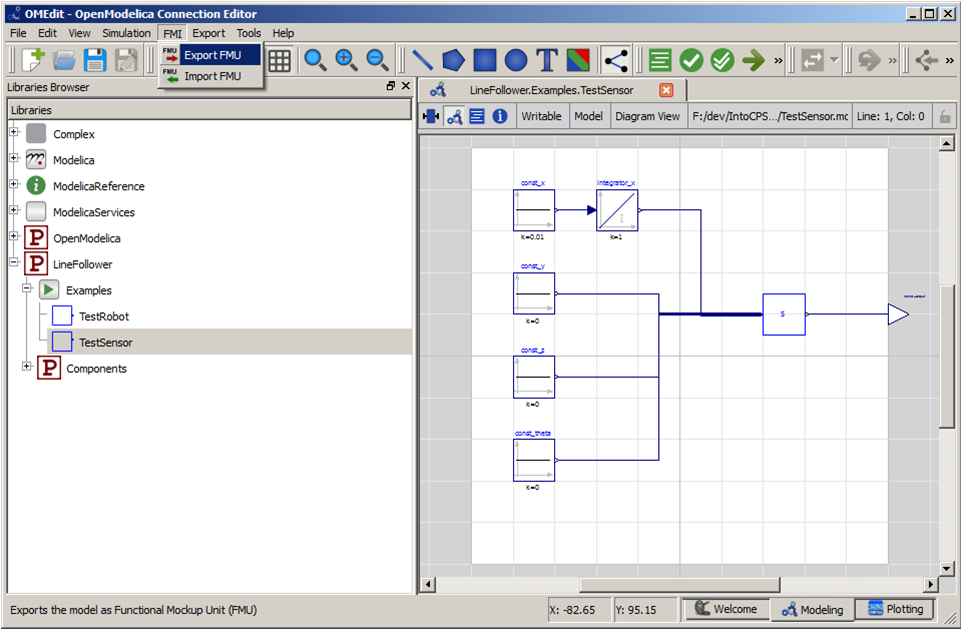
\includegraphics[width=12.5cm]{figures/OMEdit_4.png}}
	\caption{Exporting the FMU.}
	\label{figure:OMEdit_4}
\end{figure}
%
%
%
\begin{figure}[ht]
	\centerline{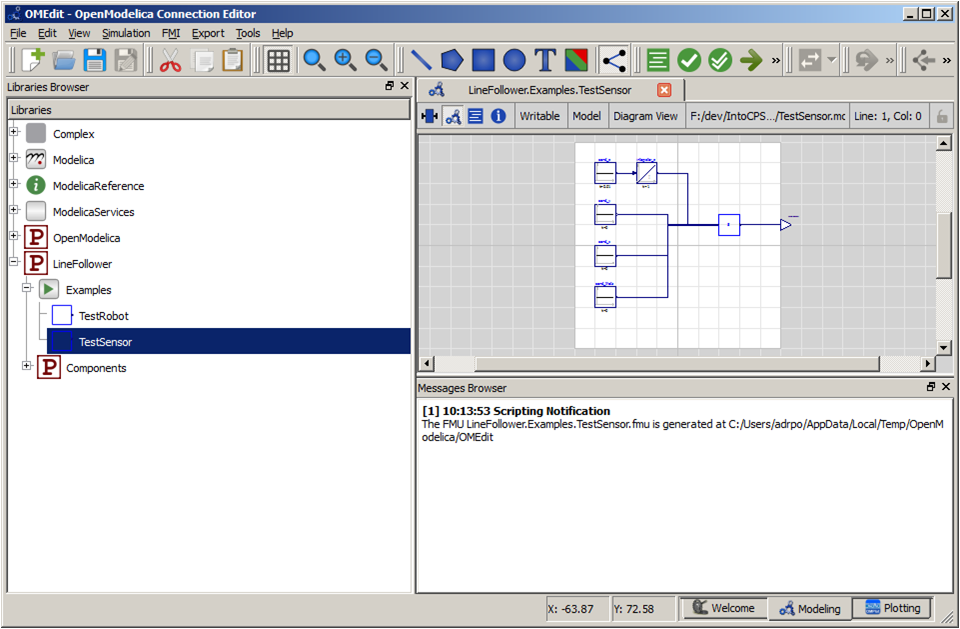
\includegraphics[width=12.5cm]{figures/OMEdit_5.png}}
	\caption{Final step of FMU export.}
	\label{figure:OMEdit_5}
\end{figure}
%
%
%
The generated FMU will be saved to \texttt{\%{}TEMP\%{}\textbackslash{}OpenModelica\textbackslash{}OMEdit}.
\clearpage
\subsection{Unity}\label{sec:simulators:unity}
This section describes the 3D visualisation functionality of the \into tool chain.
%
This capability is encapsulated into a Unity-based FMU that is configured and loaded into co-simulations in the usual manner.
%
Unity is a professional game engine.
%
It can be downloaded from the Unity website \cite{UnityWebsite}. 

\subsubsection{Importing the Unity Package into Unity}
To create a 3D animation FMU using Unity, first create a new project or open an existing Unity project. A Unity package was made by CLP that can be imported into Unity to expand Unity with FMU export options. This Unity package can be downloaded via the Download Manager in the INTO-CPS application or by contacting CLP.
%
First, drag-and-drop this package into the \textit{Assets} folder in Unity (in the \textit{Project} tab). See \autoref{figure:20-sim_import_unity_package} on how to import the package from the explorer into Unity. A pop-up will open, like the one shown in \autoref{figure:20-sim_import_unity_package_dialog}. Press the \textit{Import} button, as shown in \autoref{figure:20-sim_import_unity_package_dialog}.
%
\begin{figure}[ht]
	\centerline{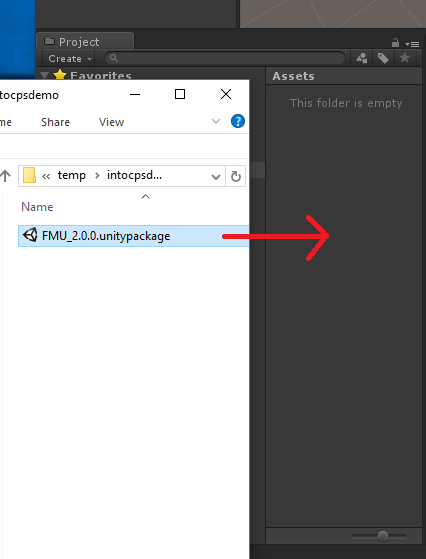
\includegraphics[width=0.6\textwidth]{figures/20sim_Unity1.png}}
	\caption{Importing the Unity package into Unity.}
	\label{figure:20-sim_import_unity_package}
\end{figure}
%
\begin{figure}[ht]
	\centerline{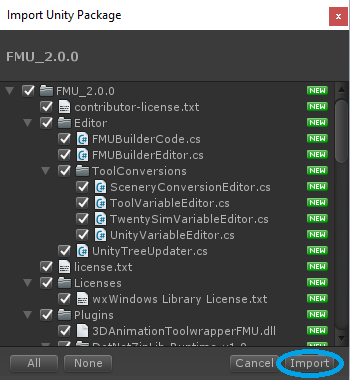
\includegraphics[width=0.4\textwidth]{figures/20sim_Unity2.png}}
	\caption{Summary of what will be imported into the Unity project.}
	\label{figure:20-sim_import_unity_package_dialog}
\end{figure}
%
Since the package contains scripts that will modify the Unity editor, it is necessary to restart the Unity project after importing the package. 
%
%
%
\subsubsection{Importing the FMUBuilder \textit{gameobject}}
After restarting Unity, go to the \textit{Hierarchy} tab. Right click within the blank part of the hierarchy (\emph{i.\@e.\@} do not select any objects in the hierarchy) and select \textit{FMU \textrightarrow FMUBuilder} (see \autoref{figure:20-sim_unity_create_fmubuilder}). This will create a new object in the hierarchy named FMUBuilder. When selecting this FMUBuilder object in the hierarchy, a few options will be shown in the \textit{Inspector} (see \autoref{figure:20-sim_unity_components_fmubuilder}). There are three components visible: \textit{Transform}, \textit{FMU Builder (Script)} and \textit{Scenery Conversion (Script)}. The latter two are unique to the INTO-CPS Unity FMU package. \textit{FMU Builder (Script)} is the component that will eventually build the 3D animation FMU, which will be covered later in this section. The other component, \textit{Scenery Conversion (Script)}, is used to convert existing 20-sim sceneries into Unity sceneries. This will also be covered later in this section.

\begin{figure}[ht]
	\centerline{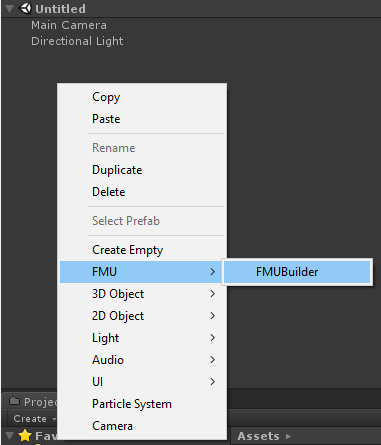
\includegraphics[width=0.5\textwidth]{figures/20sim_Unity3.png}}
	\caption{Creating the FMUBuilder \textit{gameobject} in the hierarchy tab.}
	\label{figure:20-sim_unity_create_fmubuilder}
\end{figure}

\begin{figure}[ht]
	\centerline{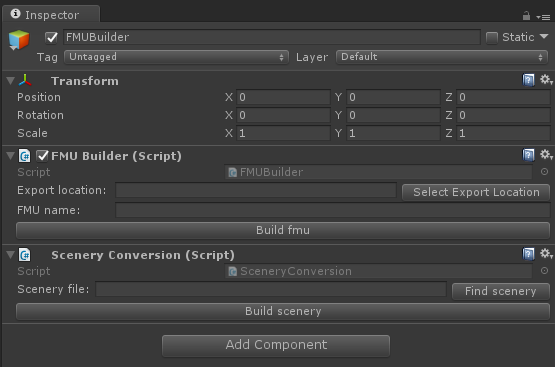
\includegraphics[width=0.7\textwidth]{figures/20sim_Unity4.png}}
	\caption{Components of the FMUBuilder in the \emph{Inspector} tab in Unity.}
	\label{figure:20-sim_unity_components_fmubuilder}
\end{figure}

\subsubsection{Assigning FMU Variables to Unity \textit{gameobject}s}
To be able to connect variables from a co-simulation to an object in Unity, a \textit{gameobject} is needed. For example, as shown in \autoref{figure:20-sim_unity_create_fmubuilder}, a cube object can be created by right-clicking in the hierarchy tab in a blank space of the hierarchy, but now selecting \textit{3D Object \textrightarrow Cube}.
%
When the newly created object is selected in the hierarchy, all components currently attached to this cube can be seen in the \textit{Inspector} tab.
%
At the bottom of this tab there is a button named \textit{Add Component}. Press this button, go to \textit{FMU variables} and choose between \textit{20-sim coordinates} or \textit{Unity coordinates}.
%
The first one means that the axes are part of a right-handed frame, that the Z-axis is pointing up, and that the order of rotation for Euler angles is X-Y-Z.
%
The latter is the Unity convention, in which the frame is left-handed, the Y-axis is pointing up, and the rotation for Euler angles is Z-X-Y.
%
See \autoref{figure:20-sim_unity_add_variable} on how to do this.
%
If there is doubt about which of the two types of variables should be chosen, choose the 20-sim option, as this is the reference frame used in most modeling tools like 20-sim.
%
Once one is selected, two additional scripts become available in the \textit{Inspector} tab. These are \textit{GUID (Script)} and either \textit{Twenty Sim Variable (Script)} or \textit{Unity Variable (Script)}. The \textit{GUID} script should not be touched. The \textit{Variable} script, however, is the script that will describe the interface variables of the to-be-generated FMU. Choose an FMU variable name and an axis, and press the \textit{Add Axis} button. Multiple axes can be defined for one \textit{gameobject}. \autoref{figure:20-sim_unity_modify_variable} shows the axes dropdown menu and the \textit{Twenty Sim Variable (Script)} and \textit{GUID (Script)} components. 

\begin{figure}[ht]
	\centerline{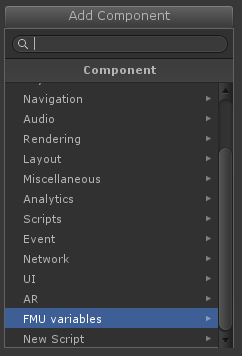
\includegraphics[width=0.4\textwidth]{figures/20sim_Unity5.png}}
	\caption{Adding new FMU variables to the Unity scene.}
	\label{figure:20-sim_unity_add_variable}
\end{figure}

\begin{figure}[ht]
	\centerline{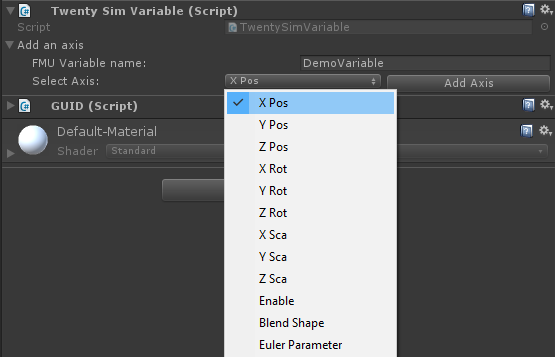
\includegraphics[width=0.7\textwidth]{figures/20sim_Unity6.png}}
	\caption{Adding the variable named "DemoVariable" for the x-position axis to the newly generated cube object.}
	\label{figure:20-sim_unity_modify_variable}
\end{figure}

\subsubsection{Converting a 20-sim Scenery into a Unity Scenery}
If a 20-sim scenery already exists, then it is possible to import it into Unity. If there is a 3D animation window in the 20-sim model, then double click the plot to open the \textit{3D Properties} window. Then go to \textit{File \textrightarrow Save Scene} (see \autoref{figure:20-sim_unity_export_scene}). If 20-sim asks to save the whole scenery, select \textit{Yes}. Remember where the scenery file is located and go back to Unity. Go to the hierarchy tab, select \textit{FMUBuilder} and enter under the \textit{Scene Conversion (Script)} the location of the scenery file, by pressing \textit{Find scenery}. Afterwards, press the \textit{Build scenery} button and the 20-sim scene will be loaded underneath the \textit{FMUBuilder} object in the hierarchy (this can be drag-dropped to other places in the hierarchy if needed), see \autoref{figure:20-sim_unity_import_scene} for the hierarchy that is created. Note that the Cube seen in \autoref{figure:20-sim_unity_export_scene} in the hierarchy is now created in Unity as well. Furthermore, the \textit{Default Lights and Cameras} frame is converted into Unity, which is a default set of lights and cameras in every 20-sim 3D scene. 
%
\begin{figure}[ht]
	\centerline{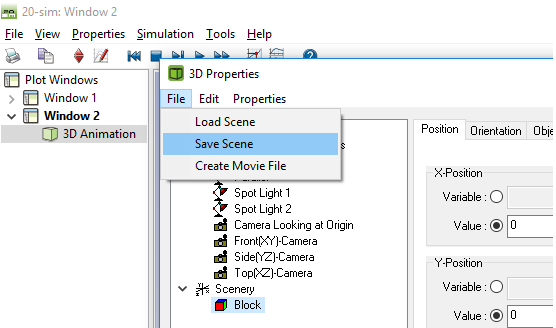
\includegraphics[width=0.7\textwidth]{figures/20sim_Unity7.png}}
	\caption{Exporting a 20-sim 3D scenery from a 3D animation plot.}
	\label{figure:20-sim_unity_export_scene}
\end{figure}
%
\begin{figure}[ht]
	\centerline{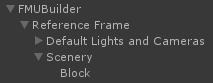
\includegraphics[width=0.3\textwidth]{figures/20sim_Unity8.png}}
	\caption{Importing a 20-sim scenery file into Unity.}
	\label{figure:20-sim_unity_import_scene}
\end{figure}
%\clearpage
%
\subsubsection{Exporting an FMU} \label{sec:simulators:20sim:fmuexport}
The final step in the process of creating a 3D animation FMU in Unity is the build process itself. The variables that were added by manually assigning FMU variables to \textit{gameobject}s and by importing 20-sim scenery files will now be used to generate the FMU itself. Every variable name (either the ones manually entered, or automatically generated by the import 20-sim scenery option) will be the input variables of this FMU. Select the \textit{FMUBuilder} in the hierarchy and go to the \textit{Inspector} tab. Under \textit{FMU Builder (Script)} select the export location and the name of the to-be-exported FMU, then press \textit{Build FMU}. Once the build process is done, the FMU will be present in the export location selected, with the given name. Note that for larger Unity scenes this can take a while to build.

\clearpage
\clearpage
\subsection{AutoFOCUS3}\label{sec:simulators:autofocus3}
AutoFOCUS3 (AF3) is an open source model based development tool for distributed, reactive and embedded software systems. It uses models to develop systems. From the requirements to the hardware architecture, passing by the design of the logical architecture, the deployment and the scheduling. It provides advanced features to support the user ensuring the quality of their system: formal analyses, synthesis methods, space exploration visualization, etc.

Co-simulation feature supports for now only Functional Mockup Unit (FMU) export satisfying the following constraints:
\begin{itemize}
  \item FMI 2.0
  \item 32/64bit
  \item GCC compilation
  \item Input and output values cannot carry NoVal but instead contain default values (0 for integers and reals, false for booleans, first item for enumerations) Note: This behavior is different from AF3 simulation
\end{itemize}

FMI export is done at the level of component with logical architecture (in the future, we might implement this feature for deployments as well). To export your component with logical architecture to the  FMU, right-click on it in the model navigator and select "Export to FMU2.0" as shown in \autoref{figure:autoFOCUSFMUExport}.

\begin{figure}[ht]
	\centerline{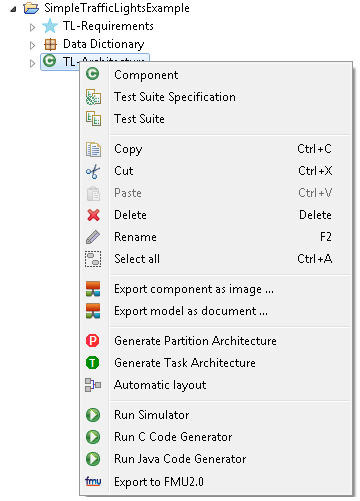
\includegraphics[width=0.6\textwidth]{figures/autoFOCUSFMUExport.png}}
	\caption{Exporting component architecture to FMU.}
	\label{figure:autoFOCUSFMUExport}
\end{figure}

AF3 works with logical time, however co-simulation is generally achieved with tools modeling reality and therefore working with real time. Therefore, the FMI standard requires that AF3 notion of time is translated to real time. Consequently, you will have to define the sampling time (in seconds) for the component as a function with name "samplingTime()" in the data dictionary as shown in \autoref{figure:autoFOCUSSamplingTime}. Otherwise, you will be asked to provide the frequency of the component in Hertz as shown in  \autoref{figure:autoFOCUSFrequency}.

\begin{figure}[ht]
	\centerline{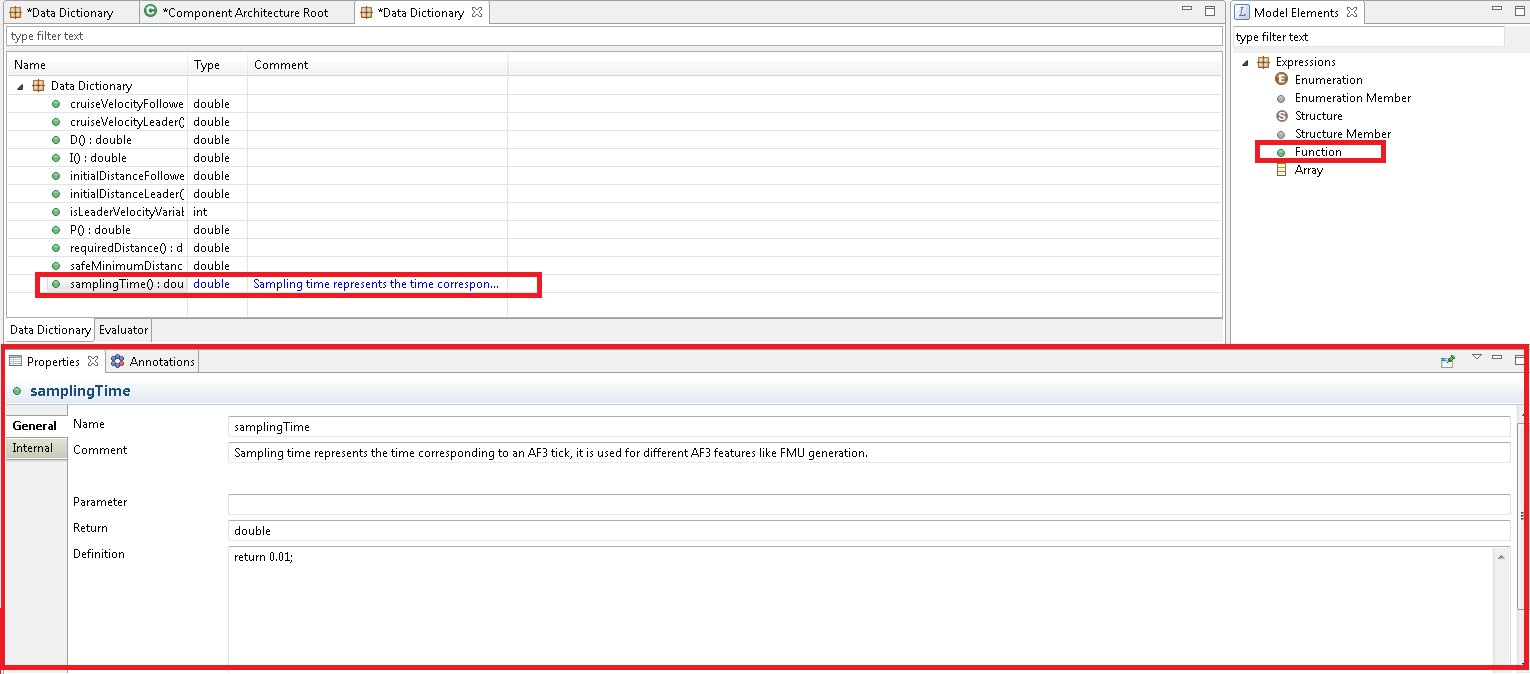
\includegraphics[width=1\textwidth]{figures/autoFOCUSSamplingTime.png}}
	\caption{Defining the sampling time function in data dictionary.}
	\label{figure:autoFOCUSSamplingTime}
\end{figure}

\begin{figure}[ht]
	\centerline{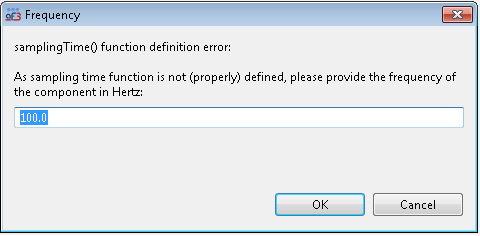
\includegraphics[width=0.6\textwidth]{figures/autoFOCUSFrequency.png}}
	\caption{Providing the component frequency in case of samplingtime() function not defined.}
	\label{figure:autoFOCUSFrequency}
\end{figure}


